\section{Methods}
\label{sec:methods}

In this manuscript, we are primarily concerned with $k$-nearest neighbors search in a finite-dimensional space.
Given a dataset $\textbf{X} = \{x_1 \dots x_n\}$, we define a \emph{point} or \emph{datum} $x_i \in \textbf{X}$ as a singular observation (e.g., the genome of 
an organism, the neural embedding of a single image, or any entity on which we can define a \emph{distance function}).

We define a \emph{distance function} $f : \textbf{X} \times \textbf{X} \mapsto \mathbb{R}^+ \ \cup \ \{0\}$ as a function which, 
given two points $x, y \in \textbf{X}$, deterministically returns a non-negative real number.
We require that the distance function be symmetric (i.e., $f(x, y) = f(y, x)$ for all $x, y \in \textbf{X}$) and that the distance between two points $x$ and $y$ be zero if and only if $x = y$. 
In addition to these constraints, if the distance function obeys the triangle inequality, i.e., it is a \emph{distance metric}, then we guarantee that CAKES has perfect recall. 
Choice of distance function varies by type of data.
For example, with electromagnetic spectra, one could both Euclidean (L2) and Cosine distances.
With biological or string data, Hamming and Levenshtein distances are more appropriate.

Some of our algorithms for $\rho$- and $k$-nearest neighbors search rely on the \emph{local fractal dimension} at some point and length scale in the dataset.
We define local fractal dimension (LFD) as:

\begin{equation}
    \frac{\text{log}(\frac{|B_X(q, r_1)|}{|B_X(q, r_2)|})}{\text{log}(\frac{r_1}{r_2}) }
    \label{eq:methods:lfd}
\end{equation}

where $B_X(q, r)$ is the set of points contained in a ball of radius $r$ centered at a point $q$ in the dataset $\textbf{X}$.
We stress that this concept differs from the \emph{embedding dimension} of a dataset.
To illustrate the difference, consider SDSS's APOGEE dataset, wherein each datum is a nonnegative real-valued vector of length 8,575.
Hence, the \emph{embedding dimension} of this dataset is 8,575. 
However, due to physical constraints (namely, the laws of physics that govern stellar fusion and spectral emission lines), the data are constrained to a lower-dimensional manifold within the 8,575-dimensional embedding space.
The \emph{local fractal dimension} is an approximation of the dimensionality of that lower-dimensional manifold in the ``vicinity'' of a given point.
This notion that high-dimensional data collected from constrained generating phenomena typically only occupy a low-dimensional manifold within their embedding space is known as the \emph{manifold hypothesis}~\cite{fefferman2016testing}.

Figures 2 and 3 in~\cite{ishaq2019clustered} illustrate the low fractal dimensions of two datasets used with $\rho$-NN search in CHESS. 
We observe that for both APOGEE (Figure 2 in~\cite{ishaq2019clustered}) and GreenGenes (Figure 3 in~\cite{ishaq2019clustered}), other than the most extreme 10\% of clusters, virtually all clusters have a local fractal dimension of less than 2. 
This suggests that APOGEE and GreenGenes are good datasets for use with entropy-scaling search algorithms like CHESS and CAKES.


\subsection{Clustering}
\label{subsec:methods:clustering}

We define a \emph{cluster} as a set of points with a \emph{center}, a \emph{radius}, and an approximation of the \emph{local fractal dimension}.
The \emph{center} is the geometric median of a sample of points in the \emph{cluster}, and so it is a real data point.
The \emph{radius} is the maximum distance from any point in the cluster to the \emph{center}.
We estimate \emph{local fractal dimension} at the scale of the cluster radius and half the cluster radius.
Each cluster (unless it is a leaf cluster) has two child clusters in much the same way that a node in a binary tree has two child nodes.
We define the \emph{metric entropy} $\mathcal{N}_{\hat{r_c}}(D)$ of a data set $D$ under a hierarchical clustering scheme as a refinement of~\cite{yu2015entropy}, where metric entropy for a given cluster radius $r_c$ was the number of clusters of radius $r_c$ needed to cover all data.
Here, we use a hierarchical, divisive clustering approach, but with early stopping criteria; clusters which satisfy a user-specified stopping criterion (e.g. a specified cardinality or radius) are not further split.
Since we frame the asymptotic complexity of $\rho$-NN search in terms of the number of leaf clusters, the \emph{metric entropy} is best thought of in terms of the number of leaf clusters.

We start by building a divisive hierarchical clustering of the dataset with CLAM, using a similar recursive procedure as outlined in CHESS, but with the following improvements:
better selection of poles for partitioning and depth-first dataset reordering (see Section ~\ref{subsubsec:methods:clustering:dataset-depth-first-reordering}). 

CAKES assumes the manifold hypothesis. 
In other words, we assume that the dataset is embedded in a $D$-dimensional space, but that the data only occupy a $d$-dimensional manifold, where $d \ll D$. 
While we sometimes use Euclidean notions, such as voids and volumes, to talk about geometric and topological properties of clusters and of the manifold, CLAM does not rely on such notions; 
they serve merely as a convenient, intuitive way to talk about the underlying mathematics.


\subsubsection {Cluster Partitioning}
\label{subsubsec:methods:cluster-partitioning}

For a cluster $C$ with $|C|$ points, we begin by taking a random sample of $\sqrt{|C|}$ of its points, and computing pairwise distances between all points in the sample.
Based on those pairwise distances, we compute the \emph{geometric median} of this sample; 
i.e., the point which minimizes the sum of distances to all other points in the sample.
This geometric median is $C$'s \emph{center}.
The \emph{radius} of $C$ is the maximum distance from any point in $C$ to its center.
The point $l$ which is responsible for that radius (i.e., the furthest point from the center) is designated the \emph{left pole}.
The point $r$ which is furthest from $l$ is designated the \emph{right pole}.
We then partition the cluster into a \emph{left child} and \emph{right child}, where the left child contains all points in the cluster which are closer to $l$ than to $r$, and the right child contains all points in the cluster which are closer to $r$ than to $l$.
Without loss of generality, we assign to the left child those points which are equidistant from $l$ and $r$.
Starting from a root-cluster containing the entire dataset, we repeat this procedure until each leaf contains only one datum or some other user-specified stopping criterion is met.
This process is described in Algorithm \ref{alg:methods:clustering:partition}.


\begin{algorithm} % enter the algorithm environment
\caption{Partition(\emph{C})} % give the algorithm a caption
\label{alg:methods:clustering:partition} % and a label for \ref{} commands later in the document
\begin{algorithmic} % enter the algorithmic environment
    \STATE $m \Leftarrow \lfloor \sqrt{|C|} \rfloor$
    \STATE $seeds \Leftarrow m$ random points from $C.points$
    \STATE $c \Leftarrow$ geometric median of $seeds$
    \STATE $l \Leftarrow \argmax d(c,x) \ \forall \ x \in C.points$
    \STATE $r \Leftarrow \argmax d(l,x) \ \forall \ x \in C.points$
    \STATE $left \Leftarrow \{x | x \in C.points \land d(l,x) \le d(r,x)\}$
    \STATE $right \Leftarrow \{x | x \in C.points \land d(r,x) < d(l,x)\}$
    \IF{$|left| > 1$}
        \STATE Partition($left$)
    \ENDIF
    \IF{$|right| > 1$}
        \STATE Partition($right$)
    \ENDIF
\end{algorithmic}
\end{algorithm}


\subsubsection {Depth-First Reordering}
\label{subsubsec:methods:clustering:dataset-depth-first-reordering}

CAKES also improves upon CHESS by reordering the dataset in depth-first order of traversal of the tree.
In CHESS, each cluster stored a list of indices into the dataset, which we used during search to retrieve a cluster's points. 
Though this approach allowed us to retrieve the points in constant time, its memory cost was prohibitively high;
since each cluster stores indices for each of its points and, for a dataset with cardinality $n$, we store a total of $n$ indices at each depth in the tree.
Assuming a balanced tree and thus $\mathcal{O}\log(n)$ depth, this approach had $\mathcal{O}(n\log(n))$ memory cost.

One may improve this memory cost to $\mathcal{O}(n)$ by only storing these indices at the leaf cluster level.
This approach, however, introduces an $\mathcal{O}(n\log(n))$ time cost whenever we need to find the indices for 
a non-leaf cluster, since it requires a traversal of the subtree rooted at that cluster.

In this work, we introduce a new approach, wherein after building the cluster tree, we reorder the dataset so that points are stored in a depth-first order.
Then, within each cluster, we need only store the cluster's cardinality and an \emph{offset} to access the cluster's points from the dataset.
The root cluster has an offset of zero and a cardinality equal to the number of points in the dataset.
A left child has the same offset as that of its parent, and the corresponding right child has an offset equal to the left child's offset plus the left child's cardinality.
With no additional memory cost nor time cost for retrieving points during search, depth-first reordering offers significant improvements over the approach used in CHESS.


\subsubsection {Scaling Behavior of Cluster Radii}
\label{subsubsec:methods:clustering:guaranteed-decrease-in-cluster-radii}

While it may be tempting to assume that cluster radii decrease with each application of Partition (refer to Algorithm \ref{alg:methods:clustering:partition}), unfortunately, this assumption is incorrect. 
Fortunately, we \emph{can} make some guarantees about the scaling behavior of cluster radii;
in particular, we prove in this section that cluster radii will stop increasing after at most $d$ partitions, where $d$ is the fractal dimensionality of the dataset. 

We can describe a $d$-dimensional distribution of data by choosing some set of $d$ mutually orthogonal axes.
Let $2R$ be the maximum pairwise distance among the points in the dataset. 
We choose the axes such that the two points that are $2R$ apart lie \emph{along one of the axes}. 
Thus, a $d$-dimensional hyper-sphere of radius $R$ would bound the dataset. 
In the worst case, (i.e., with a uniform-density distribution that fills the $d$-sphere), our axes will be such that $2R$ is the maximum pairwise distance \emph{along every axis}. 
Such a distribution would also produce a balanced cluster tree.

In this case, Partition will select a maximally distant pair of points to use as poles;
without loss of generality, say it chooses two points at the extrema one of the $d$ axes. 
After one partition, the maximum pairwise distance along that axis will be halved, i.e. bounded above by $R$.
The next recursive Partition will select another of the $d$ axes, and once again, the distance along that axis will be bounded above by $R$
Thus, after at most $d$ partitions, the maximum pairwise distance along each axis will be bounded above by $R$. 
The overall (i.e., not restricted to one axis) maximum pairwise distance 
will be bounded above by $R\sqrt{2}$ by, for example, two instances that lie at the extrema of different axes. 
See Figure~\ref{fig:methods:scaling-behavior} for an example.

Thus, starting with a cluster $C$ of radius $R$, after at most $d$ Partitions, the descendants of $C$ will each have radius
bounded above by $\frac{R}{\sqrt{2}}$. In other words, cluster radii are guaranteed to decrease by a multiplicative factor of $\frac{\sqrt{2}}{2}$ after at 
most $d$ partitions. 

Note that, in practice, we never see a balanced clustering.
Partition produces unbalanced trees due to the varying density of the sampling in different regions of the manifold and the low dimensional ``shape'' of the manifold.
Further, in practice, the cluster radii decrease by a factor much larger than $\frac{\sqrt{2}}{2}$ with almost every partition;
the upper bound of $d$ partitions is seldom realized. 

\begin{figure}[ht!]
    \centering
    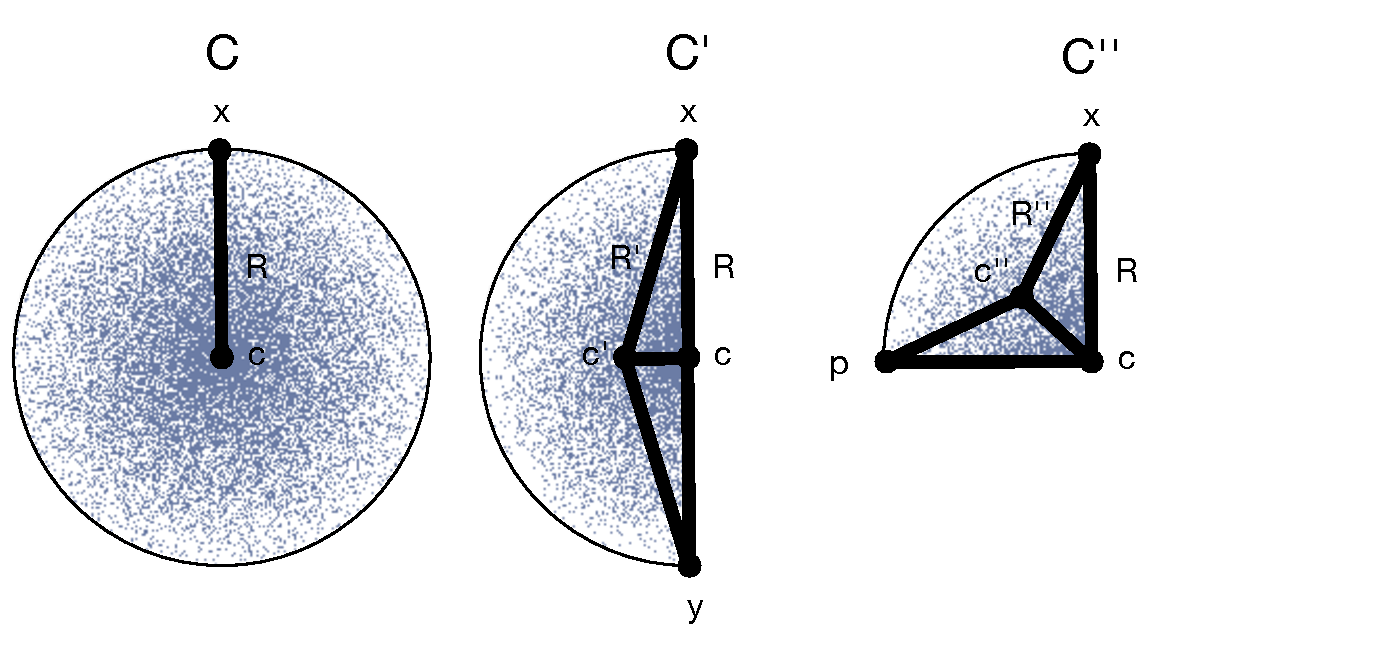
\includegraphics[width=3.4in]{images/geometry/geometry.pdf}
    \caption{
        Scaling behavior of radii on a uniform-density disk, which represents the worst-case scenario for a two-dimensional distribution. 
        $R_0$ denotes the radius of the root cluster $C_0$, and $o_0$ denotes its center. 
        After one application of Algorithm~\ref{alg:methods:clustering:partition}, we have $C_1$, with radius $R_1$ and center $o_1$.
        The right triangle formed by $o_0$, $o_1$, and $y_+$ in $C_1$ shows that $R_0 < R_1$.
        Hence, the radius of a child cluster can be larger than its parent.
        However, after another application of Algorithm~\ref{alg:methods:clustering:partition}, we have consumed all $d$ orthogonal axes, 
        as shown in $C_2$.
        Now, clearly $R_2 < R_0$.
        In fact, for each subsequent application of Algorithm~\ref{alg:methods:clustering:partition}, the radius of the resulting cluster is bounded above by $\frac{\sqrt{2}R}{2}$.
    }
    \label{fig:methods:scaling-behavior}
\end{figure}


\subsubsection {Complexity}
\label{subsubsec:methods:clustering:clustering:complexity}

The asymptotic complexity of Partition is the same as described in~\cite{ishaq2019clustered}
By using an approximate partitioning with a $\sqrt{n}$ sample, we achieve $\mathcal{O}(n)$ cost of partitioning and $\mathcal{O}(n \log n)$ cost of building the tree.
This is a significant improvement over exact partitioning and tree-building, which have $\mathcal{O}(n^2)$ and $\mathcal{O}(n^2 \log n)$ costs respectively.


\subsection {Sharding and Auto-Tuning}
\label{subsec:methods:sharding-and-auto-tuning}

In this work, we also introduce a method of \emph{sharding} for datasets that cannot fit in memory.
This approach also leverages the fact that $\rho$-nearest neighbors search at the radius of the $k$-th farthest neighbor is typically much faster than $k$-nearest neighbors search.
In addition to sharding, we perform some naive auto-tuning to select the optimal $k$-NN algorithm to be used with a given dataset.

With this approach, we begin by taking a random sample of no more than 10\% of the data.
This sample is considered the first shard.
The exact proportion of the dataset in this random sample depends on the dimensionality of the dataset and a user-specified memory limit. 
We then split the rest of the dataset into more shards based on the user-defined memory limit.
For each shard, we build a cluster tree using Algorithm~\ref{alg:methods:clustering:partition}.
From the first shard, we consider all clusters at some user-specified depth in the tree, with a default depth of 10.
Using these clusters' centers as queries, and a user-specified value of $k$, we record the time taken for $k$-NN search on the sample using each of the four algorithms described in Section~\ref{subsec:methods:knn-search}.
We select the algorithm which had the lowest total search time over all the queries. 

Sharded search then proceeds as follows.
We use previously determined $k$-NN algorithm on the first shard. 
We use the distance to the $k$-th farthest neighbor to perform $\rho$-NN search on each subsequent shard. 
After searching each shard, we keep only the $k$-nearest neighbors so far, potentially decreasing the distance to the $k$-th farthest neighbor for search on the next shard.

Note that even though we select the optimal algorithm based on use with some user-specified value of $k$, we still allow search with any value of $k$.
Note also that the size of the shards is not necessarily consistent;
it is often optimal to have the first shard be smaller than the others, since the first shard is the only one for which we perform $k$-nearest neighbors search. 
However, making this first shard too small introduces the risk of significantly overestimating the radius (i.e., the distance to the $k$-th neighbor), resulting in much slower $\rho$-nearest neighbors search on the subsequent shards.
Finding the optimal ratio between the size of the first shard and the sizes of the remaining shards, as well as computing the expected level of error between the distance from the $k$-th closest neighbor in the first shard and the actual $k$-th closest neighbor, are topics for future work.
For datasets which \emph{do} fit in memory, we use the same approach to auto-tuning, but, since the entire dataset fits in memory, there is only one shard. 


\subsection{The Search Problem}
\label{subsec:methods:the-search-problem}
Having explained the clustering process, we can now pose the $k$-NN and $\rho$-NN search problems.
Given a query $q$, along with a distance function $f$ defined on a dataset $\textbf{X}$, $k$-nearest neighbors search aims to find 
the set $S_q$ such that  $|S_q| = k$ and $\forall x \in \textbf{X} \ \setminus \ S_q$, $f(x, q) > \max\{f(y, q): y \in S_q \}$;
that is, for a given $k$, find the $k$ closest points to $q$ in $ \textbf{X}$.
We also have the $\rho$-nearest neighbors search problem, which aims to find the set $\{x \in \textbf{X}: f(q, x) \leq \rho \}$;
that is, find all points in $\textbf{X}$ that are at most a distance $\rho$ from $q$.

Given a Cluster $C$, let $c$ be its center and $r$ be its radius. Our $\rho$- and $k$-NN algorithms make use of the following properties:

\begin{itemize}
    \item $\delta = f(q, c)$ is the distance from the query to the cluster center $c$.
    \item $\delta_{max} = \delta + r$ is the distance from the query to the theoretically farthest possible instance in $C$.
    \item $\delta_{min} = \text{max}(0, \delta - r)$ is the distance from the query to the theoretically closest possible instance in $C$.
\end{itemize}

We define a \emph{singleton} as a cluster which either contains a single point (i.e., has cardinality 1) or which contains 
duplicates of the same point (i.e., has cardinality greater than 1 but contains only one unique point).
A singleton clearly has zero radius, and so $\delta_{max} = \delta = \delta_{min}$ for these clusters.
Hence, we sometimes overload the above notation to also refer to distance from a query to a point;
in these cases, we also have that $\delta_{max} = \delta = \delta_{min}$.


\subsection{\texorpdfstring{$\rho$}{p}-Nearest Neighbors Search}
\label{subsec:methods:rnn-search}

We conduct $\rho$-nearest neighbors search as described in \cite{ishaq2019clustered}, but with the following improvement:
when a cluster overlaps with the query ball, instead of  always proceeding with both of its children, we proceed only with those children which also overlap with the query ball.
This improvement is described in Algorithm \ref{alg:methods:rnn-search}.

\begin{algorithm} 
    \caption{$\rho$-NN(\emph{cluster, query, r})} 
    \label{alg:methods:rnn-search} 
    \begin{algorithmic}
        \REQUIRE $r \geq 0$
        \REQUIRE $cluster \neq \emptyset$
        \STATE $results \Leftarrow \emptyset$
        \IF{$cluster.left \cap B_X(query, r) \neq \emptyset$}
            \IF{$cluster.left.\delta$ $\leq$ $r$ + $cluster.left.radius$}
                \STATE $\rho$-NN($cluster.left, query, r$)
            \ENDIF
        \ENDIF
        \IF{$cluster.right \cap B_X(query, r) \neq \emptyset$}
            \IF{$cluster.right.\delta$ $\leq$ $r$ + $cluster.right.radius$} 
                \STATE $\rho$-NN($cluster.right, query, r$)
            \ENDIF
        \ENDIF
        \IF{$cluster.isLeaf$}
            \FOR{$p \in cluster.points$}
                \IF{$p.\delta \leq r$}
                    \STATE $results.push((p, r))$
                \ENDIF
            \ENDFOR
        \ENDIF
        \STATE Return $results$
    \end{algorithmic}
\end{algorithm}

The asymptotic complexity of $\rho$-nearest neighbors is the same as in~\cite{ishaq2019clustered}, namely:

\begin{gather}
    \mathcal{O}\Bigg(
    \underbrace{\log_2 \mathcal{N}_{\hat{r_c}}(X)}_{\textrm{metric entropy}} +
    \overbrace{\left|B_X(q,r)\right|}^{\textrm{output size}}
    \underbrace{\left(1+\frac{2\hat{r_c}}{r}\right)^d}_{\textrm{scaling factor}}\Bigg)
    \label{hierarchical-complexity}
\end{gather}

where $\hat{r_c}$ is the \textit{mean} cluster radius of leaf clusters, $\mathcal{N}_{\hat{r_c}}(X)$ is the metric entropy at that radius, $B_X(q,r)$ is a ball of data points around the query $q$ at search radius $r$, and $d$ is the fractal dimension around the query in a region of radius $r$.


\subsection{\texorpdfstring{$k$}{k}-Nearest Neighbors Search}
\label{subsec:methods:knn-search}

In this section, we present four novel algorithms for exact $k$-nearest neighbors search: $k$-NN by Repeated $\rho$-NN, Sieve Search, Sieve Search with Separate Centers, and Greedy Sieve. 
We use a preliminary auto-tuning function to predict the variant (see Section~\ref{subsec:methods:sharding-and-auto-tuning}) which will perform 
best for a given dataset and value of $k$.
We then proceed with search using that variant on the first shard. 

In these algorithms, we typically use $H$, for \emph{hits}, to refer to the data structure which stores the closest points to the query found so far and
$Q$ to refer to the data structure which stores the clusters and points which are still in contention for being one of the nearest neighbors.


\subsubsection{\texorpdfstring{$k$}{k}-NN by Repeated \texorpdfstring{$\rho$}{p}-NN}
\label{subsubsec:methods:knn-search:repeated-rnn}

In this algorithm, we perform $\rho$-nearest neighbors search starting with a small search radius, and repeatedly increasing the radius until we find $k$ neighbors.

Let $H$ be the set of nearest neighbors found thus far.
Search starts with a radius $m$ equal to the radius of the root cluster divided by the cardinality of the dataset.
We perform $\rho$-NN search with radius $m$. 
If no points are within a distance $m$ of the query, we increase the radius by a factor of 2 and perform $\rho$-NN search again, repeating until at least one point is found.

Once $|H| > 0$, we continue to perform $\rho$-NN search, but instead of increasing the radius by a factor of 2 on each iteration, we increase it by a factor determined by the local fractal dimension in the region of the dataset around the query ball. 
In particular, we increase the radius by a factor of

\begin{equation}
    \min \left(2, \left({\frac{k}{|H|}}\right)^{\frac{1}{\mu}}\right)
    \label{eq:repeated-rnn-factor}
\end{equation}

where $\mu$ is the harmonic mean of the local fractal dimensions (abbreviated lfd in algorithm below) of each cluster which contains one of the nearest neighbors found thus far.
We use the harmonic mean to ensure that $\mu$ is not dominated by outlier clusters with very high fractal dimension. 
Intuitively, the factor by which we increase the radius should be \emph{inversely} related to the number of points found so far. 
Additionally, when the local fractal dimension at the radius scale from the previous iteration is low, this suggests that the data are relatively concentrated in that region.
In other words, a small increase in the radius would likely encounter unoccupied space around the manifold, so a larger radial increase is needed.
Thus, the factor of radius increase should be \emph{directly} related to the local fractal dimension.
Once $|H| >= k$, we sort the points by their distance to the query and return the $k$ closest points.

\begin{algorithm} % enter the algorithm environment
    \caption{Repeated $\rho$-NN(\emph{root, query, k})} % give the algorithm a caption
    \label{alg:knn-by-rnn} % and a label for \ref{} commands later in the document
    \begin{algorithmic} % enter the algorithmic environment
        \STATE $H \Leftarrow$ $\emptyset$
        \STATE $m \Leftarrow$ $\frac{root.radius}{|root|}$
        \WHILE {$H = \emptyset$}
            \STATE $H.push(\rho$-NN$(root, query, m)$)
            \STATE $m \Leftarrow 2m$
        \ENDWHILE
        \WHILE {$|H| < k$}
            \STATE $Q \Leftarrow \{ C: \exists p \in H \land p \in C \}$
            \STATE $\mu \Leftarrow \frac{|Q|}{\sum_{C \in Q} \frac{1}{C.lfd}} $
            \STATE $m \Leftarrow \min \left(2, \left({\frac{k}{|H|}}\right)^{\frac{1}{\mu}}\right)$
            \STATE $H.push(\rho$-NN$(root, query, m)$)
        \ENDWHILE
        \STATE $H.sort()$
        \STATE Return $H[0 \cdots k-1]$
    \end{algorithmic}
    \end{algorithm}


\subsubsection{Complexity of \texorpdfstring{$k$}{k}-NN by Repeated \texorpdfstring{$\rho$}{p}-NN Search}
\label{subsubsec:methods:repeated-rnn-complexity}

Our complexity bounds for $k$-NN by Repeated $\rho$-NN rely on the assumption that the query point is sampled from the same distribution (i.e. arises from the same generating phenomenon) as the rest of the data.
Given the uses of $k$-NN search in practice, this assumption is not unreasonable.
From this assumption, we can infer that the local fractal dimension at the query point does not differ significantly from the mean local fractal dimension of clusters nearby the query.

We find it useful to adopt the terminology used in \cite{ishaq2019clustered} and \cite{yu2015entropy}, and address \emph{coarse search} and \emph{fine search} separately.
Coarse search refers to the process of identifying clusters which have overlap with the query ball (i.e., which are likely to contain one of the $k$ nearest neighbors). 
Fine search refers to the process of identifying the $k$ nearest neighbors among the points in those clusters identified by coarse search.

In ~\cite{ishaq2019clustered}, we claimed that the complexity of coarse search for $\rho$-NN is $\mathcal{O}(\log\mathcal{N}_{\hat{r_c}}(X))$, 
where $\mathcal{N}_{\hat{r_c}}(X)$ is the metric entropy of the dataset $X$. 
To adjust this bound for $k$-NN by Repeated $\rho$-NN, we must estimate the number of iterations of $\rho$-NN needed to find at least $k$ neighbors.

Based on the assumption that the local fractal dimension at the query point is not significantly different than that of nearby clusters, the factor from Equation \ref{eq:repeated-rnn-factor} suggests that in the expected case, we need only two iterations of $\rho$-NN to find $k$ neighbors:
one iteration to find at least one neighbor, and the one more to find enough remaining neighbors.
Since this is a constant factor, it does not affect the asymptotic complexity of coarse search, and thus we have that the complexity of coarse search for $k$-NN by Repeated $\rho$-NN is $\mathcal{O}(\log_2\mathcal{N}_{\hat{r_c}}(X))$.

To determine the asymptotic complexity of fine search, we must estimate $|F|$, the number of clusters for which we must look at all of the cluster's points.
With $\rho$-NN search, $F$ is the union of clusters which are within a distance of $r + \hat{r_c}$ from the query, where $r$ is the search radius, and $\hat{r_c}$ is the mean radius of leaf clusters, as in \cite{yu2015entropy}.
With $k$-NN by Repeated $\rho$-NN, however, the value of $r$ is dependent on the distance to the $k$th nearest neighbor, which is query-dependent.
Thus, for $k$-NN by Repeated $\rho$-NN, we adjust the definition of $F$ to be the union of clusters which are within a distance of $r' + \hat{r_c}$ from the query, where $r'$ is the distance to the $k$th nearest neighbor and $\hat{r_c}$ is defined as before.

The work in~\cite{yu2015entropy} showed that

\begin{equation*}
    |F| \leq \gamma |B(q, r')|\left(1+ \frac{2\hat{r_c}}{r'}\right)^d
\end{equation*}

where $\gamma$ is a constant. 
By definition of 
$r'$, we have that $|B(q, r')| = k$. Thus, we have that

\begin{equation}
    |F| \leq \gamma k\left(1+ \frac{2\hat{r_c}}{r'}\right)^d
    \label{eq:methods:knn-by-rnn-fine-search}
\end{equation}

It remains to provide an estimate for $r'$. 
To do this, we once again rely on the assumption that the query is from the same distribution as the rest of the data, and thus the local fractal dimension at the query point is not significantly different than that of nearby clusters.

We let $\hat{d}$ be the mean of the local fractal dimensions of the clusters near the query point (i.e., the cluster identified during coarse search).
While ordinarily we compute local fractal dimension by comparing cardinalities of two balls with two different radii centered at \emph{the same} point, in order to estimate $r'$, we instead compare the cardinality of a ball \emph{around the query} of radius $r'$ to the mean cardinality $\hat{C}$ of clusters near the query at a radius equal to the mean of their radii $\hat{r}$.
We justify this approach by noting that, since the query is from the same distribution as the rest of the data, we could replace the query with the center of one of the clusters near it without significantly changing the local fractal dimension at the query point. 

By Equation ~\ref{eq:repeated-rnn-factor}, we then have that

\begin{equation*}
    \hat{d} = \frac{\log{}\frac{\hat{C}}{k}}{\log{}\frac{\hat{r}}{r'}}
\end{equation*}

Since $\hat{d}$, $\hat{C}$, $\hat{r}$, and $k$ are all known values, we can solve equation~\ref{eq:methods:knn-by-rnn-fine-search} for $r'$ to get

\begin{equation*}
    r' = \hat{r}\left(\frac{k}{\hat{C}}\right)^{\frac{1}{\hat{d}}}
\end{equation*}

Simplifying the expression for fine search, we have that

\begin{equation*}
    k\left(1+ \frac{2\hat{r_c}}{\hat{r}}\left(\frac{k}{\hat{C}}\right)^{\frac{-1}{\hat{d}}}\right)^d
\end{equation*}

Since we are dealing with asymptotic complexity, we can ignore the additive factor of $1$.
Putting our bounds for coarse and fine search together, we have that $k$-NN by Repeated $\rho$-NN has a complexity of

\begin{equation}
    \mathcal{O}\left(\log_2{\mathcal{N}_{\hat{r_c}}(X)} + k\left(\frac{2\hat{r_c}}{\hat{r}}\right)^d\left(\frac{k}{\hat{C}}\right)^{\frac{-d}{\hat{d}}}\right)
    \label{eq:methods:knn-by-rnn-complexity}
\end{equation}

where $\mathcal{N}_{\hat{r_c}}(X)$ is the metric entropy of the dataset, $d$ is the dimensionality of the dataset, and $k$ is the number of nearest neighbors.
We note that the fraction $\frac{-d}{\hat{d}}$ should be relatively close to 1 unless fractal dimension is highly variable in a small region (that is, $\hat{d}$ differs significantly from $d$).


\subsubsection{Sieve}
\label{subsubsec:methods:knn-search:sieve}

In this algorithm, we begin by letting $Q$ be a list of clusters and points, starting with only the root cluster. 
While $Q$ contains at least one cluster (i.e., $Q$ is not a list of only points), we repeat the process described in 
the following paragraphs. 

First, we aim to find the element $q_{\tau} \in Q$ with the smallest $\delta_{max}$ such that 
$q_{\tau}$ and all elements in $Q$ with smaller $\delta_{max}$ collectively contain at least $k$ points. 

To find this element, we use a process similar to the Partition algorithm used in Quicksort~\cite{10.1093/comjnl/5.1.10}, adjusted to account for the varying cardinalities of clusters in $Q$ by having each cluster count a number of times equal to its cardinality.
Our modified version of this algorithm finds the smallest index $i$ such that all elements in $Q$ with $\delta_{max}$ less than or equal to $Q[i]$'s $\delta_{max}$ collectively have cardinality greater than or equal to $k$.
We consider $Q[i]$ to be our $q_{\tau}$, and our threshold $\tau$ to be $Q[i]$'s $\delta_{max}$.

We then remove from $Q$ any element whose $\delta_{min}$ is greater than $\tau$.
Then we remove all leaf clusters from $Q$ and add their points to $Q$ instead.
Finally, we replace all non-leaf clusters in $Q$ with their children. 

We continue this process until $Q$ contains only points.
At this point, we just use the Quicksort Partition algorithm once more to find the $k$th nearest neighbor and return all points to the left of it.

This process is described in Algorithm~\ref{alg:methods:sieve}. 

\begin{algorithm} % enter the algorithm environment
    \caption{Sieve(\emph{root, query, k})} % give the algorithm a caption
    \label{alg:methods:sieve} % and a label for \ref{} commands later in the document
    \begin{algorithmic} % enter the algorithmic environment
        \REQUIRE $root$, $query$, $k$
        \REQUIRE $root.cardinality \geq k$
        \STATE $Q \Leftarrow$ [$root$]
        \WHILE{$|Q| > k$}
            \STATE $i \Leftarrow QuicksortPartition(Q, k)$
            \STATE $\tau \Leftarrow Q[i].\delta_{max}$
            \FOR {$q \in Q$}
                \IF {$q.\delta_{min} > \tau$}
                    \STATE $Q.pop(q)$
                \ENDIF
            \ENDFOR
            \FOR {$q \in Q$}
                \IF {$q.isLeaf \lor |q| \leq k$}
                    \STATE $Q.append(q.points)$
                \ELSE
                    \STATE $[l, r] \Leftarrow q.children$
                    \STATE $Q.append([l, r])$   
                \ENDIF
                \STATE $Q.remove(q)$
            \ENDFOR 
        \ENDWHILE
        \STATE Return $Q$
    \end{algorithmic}
\end{algorithm}


\subsubsection{Sieve with Separate Centers}
\label{subsubsec:methods:knn-search:sieve2}

This algorithm is the same as Sieve, but with the following modification:
clusters in $Q$ are represented twice -- once as their center and once as the rest of their points.
The clusters' multiplicities in $Q$ are adjusted to be one less than their cardinalities.
Because we have that for any cluster $C$, $C.\delta \leq C.\delta_{max}$, representing the cluster center separately from the rest of the points causes the threshold $\tau$ to decrease more quickly, thus allowing us to eliminate some clusters from $Q$ earlier in the process. 


\subsubsection{Greedy Sieve}
\label{subsubsec:methods:knn-search:greedy-search}

We first let $Q$ be a min-queue of clusters prioritized by $\delta_{min}$.
$Q$ starts containing only the root cluster.
We also let $H$ be a fixed-size ($k$) max-queue of points prioritized by $\delta$.
$H$ starts empty.

While $H$ has fewer than $k$ points or $\delta$ of the top priority element in $H$ is greater than $\delta_{min}$ of the top priority element in $Q$, we do the following:

\begin{enumerate}
\item While the top priority element $q$ in $Q$ is not a leaf, pop it from $Q$ and push its children to $Q$.
\item For each point $p \in q$, push $p$ to $H$. 
\item Pop from $H$ until $H$ has $k$ points. 
\end{enumerate}

After this process, the points left in $H$ are the $k$ nearest neighbors of $q$.
This algorithm is described in Algorithm~\ref{alg:greedy-sieve}.

\begin{algorithm} 
\caption{Greedy Sieve(\emph{root, query, k})} 
\label{alg:greedy-sieve} 
\begin{algorithmic}
    \STATE $Q \Leftarrow$ priority queue
    \STATE $Q.push(root)$
    \STATE $H \Leftarrow$ priority queue
    \WHILE{$|H| < k \lor H.peek.\delta > Q.peek.\delta_{min}$}
        \WHILE{$\neg Q.peek.isLeaf$}
            \STATE $[l, r] \Leftarrow Q.pop().children$
            \STATE $Q.push([l, r])$
        \ENDWHILE
        \STATE $leaf \Leftarrow Q.pop()$
        \STATE $H.push(leaf)$
        \WHILE{$|H| > k$}
            \STATE $H.pop()$
        \ENDWHILE
    \ENDWHILE
    \STATE Return $H$
\end{algorithmic}
\end{algorithm}


\subsubsection{Complexity of Sieve Algorithms}
\label{paragraph:methods:sieve-complexity}

We group the Sieve-based algorithms together, as their complexity analyses are similar.
The complexity of Sieve and Sieve with Separate Centers is dominated by the expected cost of Quicksort's partition algorithm to calculate thresholds.
This method is linear in the size of the input list $Q$, so we must estimate the size of $Q$ on each iteration. 

We start by considering clusters whose cardinalities are within a small factor of $k$, say a factor of 2.
The distribution of such clusters will mimic the distribution of points in the dataset. 
From this assumption, we can infer that number of clusters which overlap with the query ball is a function of the local fractal dimension near the query.
In particular, we assume that the number of clusters which overlap the query ball is bounded above by 2$d$, where $d$ is the local fractal dimension of the dataset near the query point, e.g. we could have a cluster overlapping the query ball at each end of each of the $d$ axes.

In the worst case scenario, where the data are distributed with uniform density in their embedding space, it takes at most $\log{\frac{n}{2k}}$ iterations of Sieve to partition clusters enough that their cardinalities are at most $2k$.
However, since high cardinality clusters occur only at low depths in the tree, the length of $Q$ for those iterations is relatively low. 

After the first $\log{\frac{n}{2k}}$ iterations, we have that the cardinalities of clusters in $Q$ are at most $2k$, at which point, based on our assumption, we have that the length of $Q$ is close to $2d$.
Therefore, the asymptotic complexity of the sieve algorithms is $\mathcal{O}\left(log(\frac{n}{d})\right)$.
